\chapter{TASK\_1.}

\textbf{Цель работы:}

\begin{itemize} 
	\item 
\end{itemize}

\textbf{Задание 1}


\begin{lstlisting}[caption=Код программы. TASK\_1. Главнвая функция main]
	
\end{lstlisting}

\begin{lstlisting}[caption=Код программы. TASK\_1. Реализация заданий]
	
\end{lstlisting}


\textbf{Вывод:}

\begin{itemize} 
	\item Были изучены
\end{itemize}

\textbf{Пример работы:}

% \begin{figure}[ht!]
% 	\centering{
% 		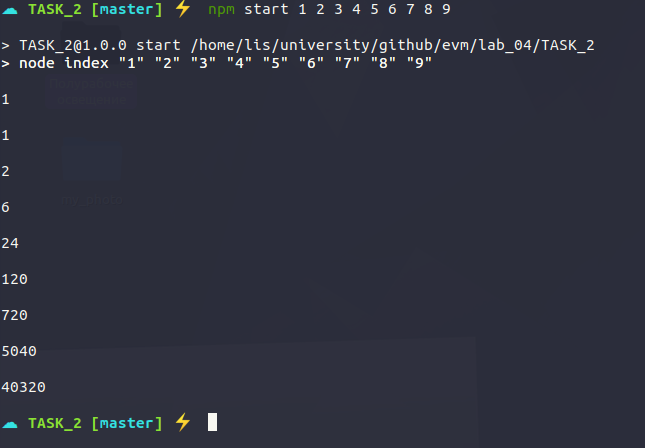
\includegraphics[width=0.9\textwidth]{img/1.png}
% 		\caption{Пример работы программы}}
% \end{figure}


\chapter{TASK\_2.}

\textbf{Цель работы:}

\begin{itemize} 
	\item Изучать и реализовать взаимодействие между серверами.
	\item Изучать и реализовать дочерние процессы.
	\item Изучать и реализовать process.argv.
\end{itemize}

\textbf{Задание 1}

Создать сервер А. На стороне сервера хранится файл с содержимым в формате JSON. При получении запроса на /insert/record идёт добавление записи в файл. При получении запроса на /select/record идёт получение записи из файла. Каждая запись хранит информацию о машине (название и стоимость).

Создать сервер Б. На стороне сервера хранится файл с содержимым в формате JSON. Каждая запись в файле хранит информацию о складе и массиве машин, находящихся на данном складе. То есть каждая запись хранит в себе название склада (строку) и массив названий машин (массив строк). При получении запроса на /insert/record идёт добавление записи в файл. При получении запроса на /select/record идёт получение записи из файла.

Создать сервер C. Сервер выдаёт пользователю страницы с формами для ввода информации. При этом сервер взаимодействует с серверами А и Б. Реализовать для пользователя функции:

создание нового типа машины
получение информации о стоимости машины по её типу
создание нового склада с находящимися в нём машинами
получение информации о машинах на складе по названию склада
Реализовать удобный для пользователя интерфейс взаимодействия с системой (использовать поля ввода и кнопки).

\textbf{Задание 2}

Написать скрипт, который принимает на вход число и считает его факториал. Скрипт должен получать параметр через process.argv.

Написать скрипт, который принимает на вход массив чисел и выводит на экран факториал каждого числа из массива. Скрипт принимает параметры через process.argv.

При решении задачи вызывать скрипт вычисления факториала через execSync.

\begin{lstlisting}[caption=Код программы. TASK\_2. Главный процесс]
	"use strict";
	
	// импортируем библиотеку
	const execSync = require('child_process').execSync;
	
	const MY_ARG = 2
	const OPTIONS = { encoding: 'utf8' };
	
	// Функция, для считывания аргументов
	// Переданных в командной строке.
	function readArgv(array) {
		let i = MY_ARG;
	
		while (process.argv[i])
			array.push(parseInt(process.argv[i++]));
	
		return array;
	}
	
	// Функция, вызывающая дочерний процесс
	// Для каждого элемента из массива array.
	// Дочерний процесс в свою очередь
	// Считает факториал числа.
	function arrayFactorial(array) {
		let cmd;
	
		for (let i in array) {
			cmd = `node factorial ${array[i]}`
			console.log(execSync(cmd, OPTIONS))
		}
	}
	
	
	function main() {
		let array = [];
		readArgv(array);
		arrayFactorial(array);
	}
	
	main();
\end{lstlisting}


\begin{lstlisting}[caption=Код программы. TASK\_2. Дочерний процесс.]
"use strict";

// Функция, которая вычисляет факториал
// Числа, переданного аргументом командной строки.
function factorial() {
	let num = parseInt(process.argv[2]);
	let result = 1;

	for (let i = 1; i < num; i++)
		result *= i;

	console.log(result);
}

factorial();
\end{lstlisting}

\begin{lstlisting}[caption=Код программы. TASK\_2. Главный файл]
\end{lstlisting}


\textbf{Вывод:}

\begin{itemize} 
	\item Мы изучили и реализовали взаимодействие между серверами.
	\item Изучили и реализовали дочерние процессы.
	\item Изучили и реализовали process.argv.
\end{itemize}


\textbf{Пример работы:}

\begin{figure}[ht!]
	\centering{
		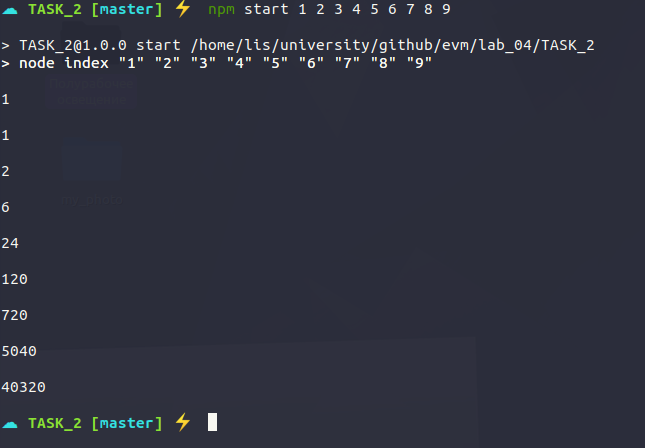
\includegraphics[width=0.9\textwidth]{img/1.png}
		\caption{Пример работы программы}}
\end{figure}
